\subsubsection{Card con los tops de la empresa}
Esta Card, en el encabezado, tiene dos pestañas que mostrarán tops diferentes. La pestaña por defecto es la que lleva por título ``Productos'', y en esta se muestra un gráfico llamado Treemap que muestra los datos jerárquicamente en forma de rectángulos anidados.

En esta Card también se encuentran los botones que permiten manipular la gráfica mediante el formato de moneda o cantidad. El formato por defecto es el de moneda (Ver Figura 33): 

    \begin{figure}[H]
        \begin{center}
            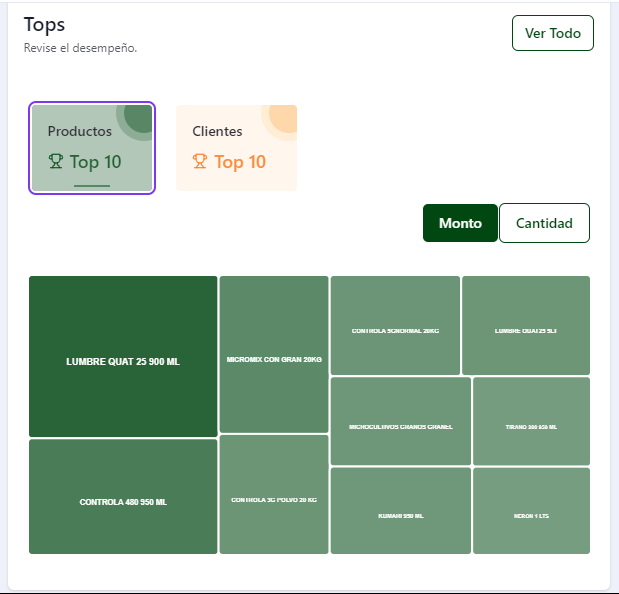
\includegraphics[scale=0.40]{img/actividades/dahsboard-admin/top-producto-monto.png}
            \caption{Gráfica treemap de productos con formato de moneda.}
            \label{fig:top-producto-monto}
        \end{center}
    \end{figure}

El gráfico mostrará 10 rectángulos con los 10 productos que le generan mayores ingresos a la empresa. Los rectángulos tendrán el nombre del producto y al pasar el cursor sobre ellos, se podrán ver los ingresos.

Al cambiar el formato a cantidad, el aspecto de la gráfica cambiará pues se está utilizando otro conjunto de datos para renderizarla. La gráfica volverá a mostrar 10 rectángulos con los 10 productos de los cuales se ha vendido mayor cantidad, y esto también provocará que la jerarquía de los rectángulos cambie (Ver Figura 34).

    \begin{figure}[H]
        \begin{center}
            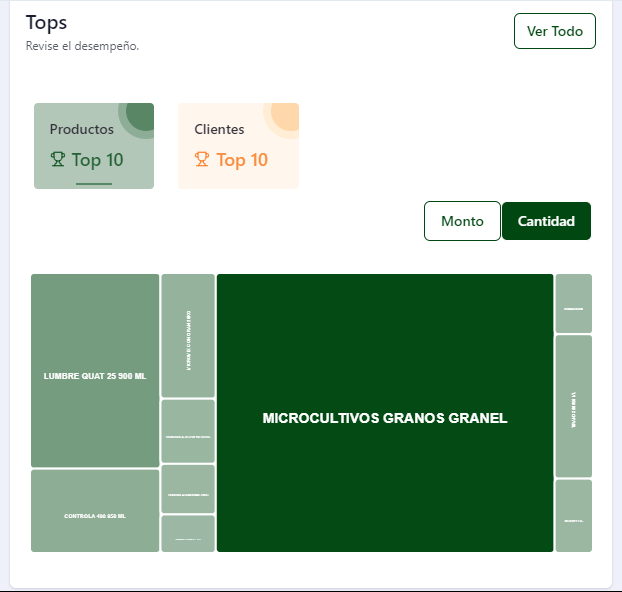
\includegraphics[scale=0.40]{img/actividades/dahsboard-admin/top-producto-cantidad.png}
            \caption{Gráfica treemap de productos con formato de cantidad.}
            \label{fig:top-producto-cantidad}
        \end{center}
    \end{figure}

Lo mismo ocurrirá al cambiar a la pestaña de clientes, sólo que ahora se mostrará quienes son los 10 clientes que generan más ingresos para Mezfer (Ver Figura 35):

    \begin{figure}[H]
        \begin{center}
            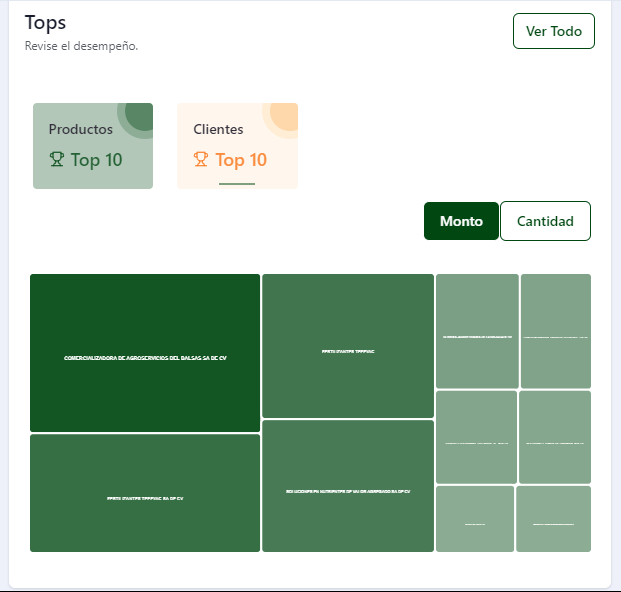
\includegraphics[scale=0.40]{img/actividades/dahsboard-admin/top-clientes-monto.png}
            \caption{Gráfica treemap de clientes con formato de monto}
            \label{fig:top-cliente-monto}
        \end{center}
    \end{figure}